\chapter{Mortality in individuals treated with glucose lowering agents: a large, controlled cohort study}\label{ch:survival}

\chapterfrontpagesubmitted{
Claesen, M.$^\star$, Gillard, P.$^\star$, De Smet, F., Callens, M., De Moor, B. \& Mathieu, C. (2015). 
\textbf{Mortality in individuals treated with glucose lowering agents: a large, controlled cohort study},
\emph{Journal of Clinical Endocrinology and Metabolism}.\\
$^\star$: these authors have contributed equally to the manuscript.
}{
Marc Claesen contributed to the study design and performed all data extractions and statistical analyses.
}{
\paragraph{Context} Several observational studies and meta-analyses have reported increased mortality of patients taking sulfonylurea and insulin. The impact of patient profiles and concomitant therapies often remains unclear. 

\paragraph{Objective} To quantify survival of patients after starting glucose-lowering agents (GLAs) and compare it to control subjects, matched for risk profiles and concomitant therapies.

\paragraph{Design} Controlled, retrospective cohort study. 

\paragraph{Setting} The study is based on health expenditure records of the largest Belgian health mutual insurer, covering over 4.4 million people.
Patients: 115,896 patients starting metformin, sulfonylurea or insulin (alone or in combination) between January 2003 and December 2007. Control subjects without GLA therapy were matched for age, gender, history of cardiovascular events and therapy with antihypertensives, statins and blood platelet aggregation inhibitors.

\paragraph{Main Outcome Measure} 5-year survival after start of GLA. 

\paragraph{Results} Profiles of patients using different GLAs varied, with patients on sulfonylurea being oldest and patients on insulin having more frequently a history of cardiovascular disease. Excess mortality differed across GLA therapies compared to matched controls without GLAs, even after adjusting for observable characteristics. Only metformin monotherapy was not associated with increased 5-year mortality compared to matched controls, while individuals on combination of sulfonylurea and insulin had highest mortality risks. Age and concomitant use of statins strongly affect survival. 

\paragraph{Conclusions} Differences exist in 5-year survival of patients on GLA, at least partly driven by the risk profile of the individuals themselves. Metformin use was associated with lowest 5-year mortality risk and statins dramatically lowered 5-year mortality throughout all cohorts.
}



%%%%%%%%%%%%%%%%%%%%%%%%%%%%%%%%%%%%%%%%%%%%%%%%%%
% Keep the following \cleardoublepage at the end of this file, 
% otherwise \includeonly includes empty pages.
\cleardoublepage

\section{Introduction}
Glucose lowering therapy in type 2 diabetes is challenging, due to the progressive nature of the disease by the underlying failure of the insulin-secreting beta-cells \citep{s1}. Algorithms and guidelines are proposed by international bodies, guiding clinicians through the maze of possibilities of glucose-lowering agents, but guidance is mostly based on evidence from the original UKPDS study, reported in the middle of the 1990's \citep{s2}. Evidence on the impact of glucose-lowering agents on the hardest endpoint, survival, is limited. In particular, sulfonylurea and insulin have been associated with higher mortality risks in cross-sectional studies or population studies \citep{s3,s4,s5,s6,s7,s8} with criticisms arising that comparing the mortality risk in these individuals to the global population is unfair as the profile of this population may be different, predisposing them to a higher mortality risk. On the other hand, many studies report a lower mortality risk in type 2 diabetes patients treated with metformin \citep{s3,s4,s5,s6,s7,s8,s9} but again, the profile of these people may be different by itself, thus influencing risk. Finally, in the high cardiovascular risk disease that is type 2 diabetes, use of statins has been debated frequently, with doubts being cast over the usefulness of these drugs in this population, in particular in the young or very old age groups. 

This study investigated the survival of patients starting therapies involving various glucose-lowering agents (GLAs) compared to fully matched control subjects. We particularly analyzed the effect of age and concomitant use of statins.

This study was performed in collaboration with the largest mutual health insurance fund in Belgium (National Alliance of Christian Mutualities - NACM), which has access to a large database containing health expenditure records of 4.4 million people throughout the country. The Belgian health care insurance is a broad solidarity-based form of social insurance. Mutual health insurers like NACM are the legally-appointed bodies for managing and providing the Belgian compulsory health care and disability insurance. To implement its operations, NACM disposes of a large database containing health expenditure records of all its members. These records hold all financial reimbursements of drugs, procedures and contacts with health care professionals. Long-term follow-up and full matching of the people using GLAs to people identical in age, gender, concomitant medications and start of follow-up are possible. We performed a 5-year survival analysis to assess the excess mortality in patient cohorts defined by their GLA therapy compared to references without GLA therapy but with otherwise similar observable characteristics. Our analysis shows differences in 5-year survival in individuals treated with GLAs, at least partly driven by the risk profile of the individuals themselves. 

\section{Research design and methods}

This study is based on records of the NACM, the largest Belgian mutual health insurer with over 4.4 million members (market shares of over 40\% and 60\% in Belgium and Flanders, respectively). All data extractions and analyses were performed at the Medical Management Department of the NACM under supervision of the Chief Medical Officer.
NACM disposes of a longitudinal overview of its members' medical resource use, embedded in health expenditure records. Only 2\% of the subpopulation under study left the NACM to switch to another mutual health insurer, emigration or employment by a foreign employer during the 5-year follow-up period, leading to a retention rate of 98\% in our study. Patients that joined NACM after December 1999 were excluded from all analyses to minimize the chance of missing glucose-lowering therapy and/or cardiovascular events prior to starting follow-up.

Medication records were mapped onto the fifth level of the anatomical therapeutic chemical (ATC) classification system via the main chemical substances associated with each drug. The ATC system classifies drugs based on the targeted organ or system and their therapeutic and chemical characteristics \citep{s10}. Patients were partitioned into treatment groups based on ATC codes listed in their individual histories. Exact definitions of all pharmacological groups can be consulted in Table~\ref{table:survival-defs}. In addition to pharmacotherapy, we considered a set of cardiovascular events prior to follow-up, which were identified via a combination of medicinal and surgical interventions (also described in Table~\ref{table:survival-defs}). Based on usual prescription behavior in Belgium, exposure of oral glucose lowering drugs was assumed to be uninterrupted between the dates of the first record and up to six months after the final record in the insurance database. 

\begin{table}[!h]
\begin{tabular}{p{0.2\textwidth}p{0.78\textwidth}}
\toprule
Category        & Definition \\
\midrule
metformin       & ATC codes: A10BA02, A10BD02, A10BD07, A10BD08 \\
sulfonylurea    & ATC codes: A10BB01, A10BB08, A10BB09, A10BB12, A10BD02 \\
insulin         & ATC codes: A10AB02, A10AB03, A10AB04, A10AB05, A10AB06, A10AB30, A10AC01, A10AC02, A10AC03, A10AC04, A10AC30, A10AD01, A10AD02, A10AD03, A10AD04, A10AD05, A10AD30, A10AE01, A10AE02, A10AE03, A10AE04, A10AE05, A10AE30, A10AF01 \\
statins         & ATC codes: all codes under C10AA \\
antihypertensives       & ATC codes: all codes under C02, C03, C07, C08, C09 \\
blood platelet aggregation inhibitors & ATC codes: all codes under B10AC \\
\midrule
cardiovascular events & An arterial thrombotic event of the coronary, carotid, vertebral, aortic, iliac or lower extremity arteries necessitating an intervention for revascularization. Open and/or percutaneous interventions included thrombectomy, embolectomy, endarterectomy, artery bypass, vascular endoprosthese, endovascular dilatation, stenting or brinolysis. A positive history of a cardiovascular event was defined as having one or more of those events reimbursed by the NACM based on the Belgian nomenclature of health care provisions. \\
\bottomrule
\end{tabular}
\caption{Definitions of drug categories and cardiovascular events.} \label{table:survival-defs}
\end{table}


\subsection{Study cohort selection}
The selection process is illustrated in Figure~\ref{fig:survival-selection}. 115,896 patients over 18 years old in whom glucose-lowering therapy was prescribed between 1st of January 2003 and 31st of December 2007 were eligible for the study. Eligible patients were assigned to study cohorts based on their glucose-lowering pharmacotherapy: more specifically metformin (MET), sulfonylurea (SU) and insulin (INS). Every combination of these three drug types defines a study cohort. Patients on DPP4 inhibitors or GLP-1 receptor agonists were not included as these were only introduced in Belgium around 2008. 

\begin{figure}[!p]
  \centering 
      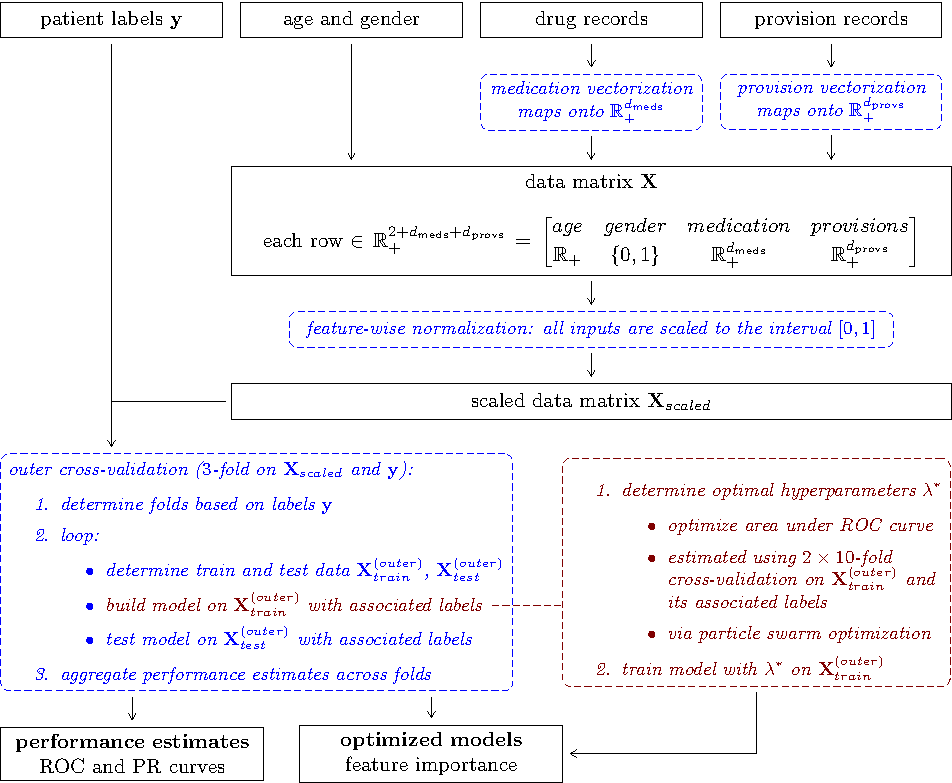
\includegraphics[width=\textwidth]{flowchart.pdf} 
  \caption{Flowchart describing the selection protocol for study and control patients. Patients can move
from the bottom right (monotherapy) to the bottom left group (combination therapy), but not vice
versa. All listed counts are for unique patients.}\label{fig:survival-selection}
\end{figure}

Follow-up started on the first day of therapy intake, based on the patient's purchase of the prescribed agent(s). In each study and control group, subjects were followed until death or censoring over a maximum period of 5 years since inclusion. For control subjects, the start of follow-up was determined at random within the year of inclusion of the associated study patient to avoid bias related to the time of entry into the study.

Monotherapy study cohorts denote the first glucose-lowering therapy consisting of a single type of GLA, given to a patient without prior use of other GLAs (n=74,938), based on historical records from 1990 onwards. Patients are excluded from monotherapy cohorts if they transition to combination therapy within three months. Patients who started a combination therapy during the selection interval for at least 3 months (or until death) were included in the associated study cohorts, regardless of potential prior glucose-lowering therapy (n=47,149). 

Patients could successively enter multiple study cohorts and be included in multiple cohorts during follow-up. For instance, a patient without prior GLA therapy who started metformin in 2003 and added sulfonylurea in 2005 is included in both the metformin monotherapy and the metformin and sulfonylurea combination therapy cohorts (5-year follow-up starting in 2003 and 2005, respectively), with some period of overlap (2005-2008).  

Only patients with at least one month between the first and last purchase of associated GLAs were included in study cohorts, inducing an immortal time of one month. We accounted for potential bias by consistently matching control patients who survived for at least one month \citep{s11,s12}. Patients who started treatment and died during a single hospital admission were excluded from the analysis. 

\subsection{Control cohort selection}
We compared study groups to controls with similar observable characteristics. Controls were sampled without replacement from the NACM population with matched characteristics to the study cohort, but without records of GLA therapy up to and including 2013.  
Unless stated otherwise, the control groups contained 5 subjects per subject in the study cohort, matched exactly on age at the start of follow-up, gender, cardiovascular history (had event/no event before the start of the follow-up), associated therapy (use of statins, antiplatelet and antihypertensive drugs) and the year of start of follow-up. Matching based on associated therapy was performed dichotomously (subject has/has not received the therapy for more than half of the individual's effective follow-up period).

\subsection{Therapy changes within cohorts}
The majority of patients remained on the same GLA therapy during the entire follow-up (Table~\ref{table:survival-transitions}). 15.4 to 28.5\% of patients starting on monotherapy moved to a combination therapy by the end of the follow-up. Patients on combination therapy at start were still on the same regimen in 47.7 to 66.5\% of cases: changes were often due to stopping of sulfonylurea (9 to 20\%) or eliminating metformin from combination regimens that include insulin (15.2 to 18.7\%). 

\afterpage{%
    \clearpage% Flush earlier floats (otherwise order might not be correct)
    \thispagestyle{empty}% empty page style (?)
    \begin{landscape}% Landscape page
        \centering % Center table
\begin{tabular}{lccclcccc}
\toprule
						 		& \multicolumn{3}{c}{mono therapy} & & \multicolumn{4}{c}{combination therapy} \\\cline{2-4} \cline{6-9}
$\rightarrow$ end regimen		& metformin & sulfonylurea 	& insulin 	& 	& metf+sulf & metf+ins 	& sulf+ins 	& metf+sulf+ins \\
\midrule
%\multicolumn{5}{l}{\textbf{overview categories}} \\
%any OAD	or insulin				& $37.3\%$ & $12.7\%$ & $10.8\%$ & & $14.4\%$ & $4.1\%$ & $2\%$ & $2.4\%$ & $16.4\%$ \\
%any OAD							& $44.4\%$ & $14.9\%$ & $1.7\%$ & & $17\%$ & $3.1\%$ & $1.5\%$ & $2.3\%$ & $15.1\%$ \\
%\multicolumn{5}{l}{\textbf{mono therapy}}	\\
metformin						& $81.8\%$ & $2.0\%$ & $0.8\%$ & & $10.9\%$ & $2.9\%$ & $0.3\%$ & $1.3\%$ \\
sulfonylurea					& $5.2\%$ & $63.9\%$ & $2.4\%$ & & $20.7\%$ & $1.3\%$ & $3.9\%$ & $2.7\%$ \\
insulin							& $2.2\%$ & $0.9\%$ & $86.2\%$ & & $0.7\%$ & $5.8\%$ & $2.6\%$ & $1.6\%$ \\
%\multicolumn{5}{l}{\textbf{combination therapy}}	\\
metf+sulf						& $9.2\%$ & $4.5\%$ & $3.2\%$ & & $66.5\%$ & $5.5\%$ & $1.7\%$ & $9.3\%$ \\
metf+insulin					& $9.5\%$ & $0.5\%$ & $15.2\%$ & & $1.9\%$ & $66.1\%$ & $1.3\%$ & $5.5\%$ \\
sulf+insulin					& $0.9\%$ & $11.2\%$ & $20.1\%$ & & $2.9\%$ & $3.2\%$ & $51.6\%$ & $10.2\%$ \\
metf+sulf+insulin				& $2.3\%$ & $1.7\%$ & $11.7\%$ & & $9.1\%$ & $20.6\%$ & $7.0\%$ & $47.7\%$ \\
\bottomrule
\end{tabular} \label{table:survival-transitions}
\captionof{table}{Partitioning of final treatment regimen of patients starting a specific therapy (rows). The final treatment regimen (columns) is based on the last 9 months of individual followup. Patients are censored in all survival analyses after 9 consecutive months of renunciation from metformin, sulfonylurea and insulin.}
\end{landscape}
\clearpage%
}


\subsection{Censoring}
As we were primarily interested in prognoses for patients starting a certain therapy, no censoring was done based on therapy changes (such as adding additional GLAs) or poor compliance. Censoring based on therapy changes would be informative and hence bias the survival estimates of interest. Patients that discontinued all GLA therapy for nine consecutive months are right censored, as this was considered to indicate that the patient was not using GLAs to manage glucose levels (e.g. using metformin for weight loss). Right censoring also occurred when subjects left the health insurer (lost to follow-up), which was rare (less than 2\% of all patients in follow-up in each cohort). Switching health insurer was considered unrelated to a patient's medical condition and can therefore be considered non-informative.

\subsection{Statistical analysis}
Empirical survival curves were obtained using the Kaplan-Meier estimator. The associated 95\% CIs were computed using the exponential Greenwood formula \citep{s13}. 
We used Cox proportional hazards (PH) models to quantify excess mortality between study and control cohorts while controlling for all observable patient characteristics. Adjusting for concomitant medication was particularly important, as controls were only matched in a binary fashion. Unless mentioned otherwise, the PH models contained the following set of predictors: continuous covariates describing age at start of follow-up and associated therapy (specifically statins, antiplatelet and antihypertensive drugs) and dichotomous factors for gender and the group a subject belonged to (study or control). Associated therapy-related predictors quantify the fraction of the subject's effective follow-up time during which he/she was exposed to the agent. Finally, an interaction term between age and gender is consistently included. 
The PH assumption was assessed via the Grambsch-Therneau test on scaled Schoenfeld residuals from the PH models \citep{s14}. The proportionality assumption was tested for each reported hazard ratio at the 1\% significance level and rejections are indicated in all tables. 

\paragraph{Software}
Statistical analyses were conducted in R using the survival package \citep{s15,s16}. Statistical plots were made in R using the ggplot2 package \citep{s17}.

\section{Results}

\subsection{Baseline cohort characteristics}
An overview of the study cohorts and their baseline characteristics is given in Table~\ref{table:survival-baseline}. The study group with the youngest patient population was the group on insulin monotherapy without CV history (p < 0.001 compared to all other groups), followed by patients on metformin monotherapy without CV history (p < 0.001 compared to all remaining groups). The oldest patients were those who received sulfonylurea regardless of CV history (p < 0.001 compared to all other groups). Patients with a history of CV disease were consistently older than others (p < 0.001 in all pair-wise comparisons to groups without CV history) except in the sulfonylurea-insulin combination group. 
Patients without insulin in their GLA therapy were less likely to have a history of CV disease (less than 9\% percent of the total group) than patients with insulin on board (more than 20\% percent of total group) (p < 0.001). 

\afterpage{%
    \clearpage% Flush earlier floats (otherwise order might not be correct)
    \thispagestyle{empty}% empty page style (?)
    \begin{landscape}% Landscape page
        \centering % Center table
\resizebox{1.2\textwidth}{!}{
\begin{tabular}{lrrrrrr}
\toprule
 		&   & 			& gender 		&  \multicolumn{3}{c}{associated therapy} \\\cline{5-7} 
 		&  subjects & age 			& female 		& statins 		& antiplatelet	& antihypertensive 		\\
study cohort	&  $n$	&	$mean \pm SD$		& $n$ ($\%$)	& $n$ ($\%$)	& $n$ ($\%$)				& $n$ ($\%$)	\\
\midrule
\rowcolor[gray]{.90}
metformin                       & $42,900$ & $62.0\pm12.3$ & $21,759$ ($51$) & $19,747$ ($46$) & $7,725$ ($18$) & $33,785$ ($79$) \\
$\quad$ no cv history 			& $39,578$ & $61.6\pm12.4$ & $20,913$ ($53$) & $17,127$ ($43$) & $5,579$ ($14$) & $30,592$ ($77$) \\
$\quad$ cv history				& $3,322$ & $66.8\pm10.3$ & $846$ ($25$) & $2,620$ ($79$) & $2,146$ ($65$) & $3,193$ ($96$) \\

\rowcolor[gray]{.90}
sulfonylurea					& $19,231$ & $68.4\pm12.6$ & $10,100$ ($53$) & $7,479$ ($39$) & $3,825$ ($20$) & $15,507$ ($81$) \\
$\quad$ no cv history 			& $17,438$ & $68.0\pm12.8$ & $9,576$ ($55$) & $6,325$ ($36$) & $2,739$ ($16$) & $13,786$ ($79$) \\
$\quad$ cv history				& $1,793$ & $71.8\pm9.7$ & $524$ ($29$) & $1,154$ ($64$) & $1,086$ ($61$) & $1,721$ ($96$) \\

\rowcolor[gray]{.90}
insulin							& $12,807$ & $62.8\pm17.8$ & $5,818$ ($45$) & $3,842$ ($30$) & $4,270$ ($33$) & $10,214$ ($80$) \\
$\quad$ no cv history			& $10,372$ & $61.0\pm18.7$ & $5,125$ ($49$) & $2,395$ ($23$) & $2,410$ ($23$) & $7,827$ ($75$) \\
$\quad$ cv history 				& $2,435$ & $70.6\pm10.2$ & $693$ ($28$) & $1,447$ ($59$) & $1,860$ ($76$) & $2,387$ ($98$) \\

%\multicolumn{5}{l}{\textbf{combination therapy}} \\
\rowcolor[gray]{.90}
metf+sulf						& $25,218$ & $65.8\pm12.0$ & $12,632$ ($50$) & $11,718$ ($46$) & $5,521$ ($22$) & $20,913$ ($83$) \\
$\quad$ no cv history 			& $22,830$ & $65.4\pm12.1$ & $11,966$ ($52$) & $9,973$ ($44$) & $4,038$ ($18$) & $18,612$ ($82$) \\
$\quad$ cv history				& $23,88$ & $69.6\pm9.4$ & $666$ ($28$) & $1,745$ ($73$) & $1,483$ ($62$) & $2,301$ ($96$) \\

\rowcolor[gray]{.90}
metf+insulin					& $9,506$ & $64.8\pm13.9$ & $4,880$ ($51$) & $4,891$ ($51$) & $3,562$ ($37$) & $8,305$ ($87$) \\
$\quad$ no cv history 			& $7,874$ & $64.0\pm14.5$ & $4,330$ ($55$) & $3,716$ ($47$) & $2,333$ ($30$) & $6,710$ ($85$) \\
$\quad$ cv history				& $1,632$ & $68.7\pm10.1$ & $550$ ($34$) & $1,175$ ($72$) & $1,229$ ($75$) & $1,595$ ($98$) \\

\rowcolor[gray]{.90}
sulf+insulin					& $6,087$ & $74.1\pm11.0$ & $3,201$ ($53$) & $2,285$ ($38$) & $2,730$ ($45$) & $5,580$ ($92$) \\
$\quad$ no cv history			& $4,580$ & $74.1\pm11.6$ & $2,639$ ($58$) & $1,415$ ($31$) & $1,584$ ($35$) & $4,108$ ($90$) \\
$\quad$ cv history 				& $1,507$ & $74.1\pm8.8$ & $562$ ($37$) & $870$ ($58$) & $1,146$ ($76$) & $1,472$ ($98$) \\

\rowcolor[gray]{.90}
metf+sulf+insulin				& $10,653$ & $69.1\pm11.4$ & $5,570$ ($52$) & $5,405$ ($51$) & $4,680$ ($44$) & $9,746$ ($91$) \\
$\quad$ no cv history			& $8,380$ & $68.7\pm12.0$ & $4,800$ ($57$) & $3,827$ ($46$) & $2,933$ ($35$) & $7,520$ ($90$) \\
$\quad$ cv history 				& $2,273$ & $70.5\pm9.1$ & $770$ ($34$) & $1,578$ ($69$) & $1,747$ ($77$) & $2,226$ ($98$) \\
\bottomrule
\end{tabular} \label{table:survival-baseline}
}
\captionof{table}{\footnotesize Baseline characteristics of the study cohorts. Individuals starting starting mono therapy are selected such that they have no prior history of diabetes-related drugs. Individuals starting combination therapy may have a prior history of diabetes-related drugs. All differences in use of associated therapy are statistically significant between study cohorts, except for use of antihypertensives in insulin and sulfonylurea mono cohorts (no significant difference). All associated therapy use is statistically significantly elevated in subgroups with prior cardiovascular events within each study cohort. All comparisons of study group characteristics use significance level $\alpha=0.05$ and are computed using Tukey's test in conjunction with ANOVA to adjusts for multiple comparison.}
\end{landscape}
\clearpage%
}

The percentage of males and intake of associated therapies (statins, antiplatelet and antihypertensive therapies) were consistently higher in the patients with a history of CV disease than in those without, irrespective of the glucose lowering therapy (p < 0.001 for all groups). The majority of patients with a CV history were taking statins for over half the follow-up period, ranging from 58\% in the SU + INS group to 79\% in the metformin monotherapy group. In contrast, only a minority of patients without CV history were taking statins: ranging from 23\% in the insulin monotherapy group to 47\% in the MET + INS group. 

\subsection{Five-year survival in individuals on different glucose lowering agents}
Compared to their associated matched controls, patients on metformin monotherapy showed no significant excess mortality during the follow-up. In contrast, patients started on SU, and certainly on insulin, did much worse than their respective controls (Figure~\ref{fig:survival-curves}). The excess mortality was highest in patients starting on insulin (23.8\%), followed by SU (4.1\%) and finally metformin (0.3\%, though not statistically significant at the 5\% significance level). Patients who started with bitherapy (MET + SU or MET + INS) or tritherapy (MET +SU +INS) also exhibited reduced 5-year survival compared to matched controls, with the highest difference in survival (12.9 and 15.6\%) when insulin was part of the regimen from the start of follow-up. 

\begin{figure}[h]
  \centering
  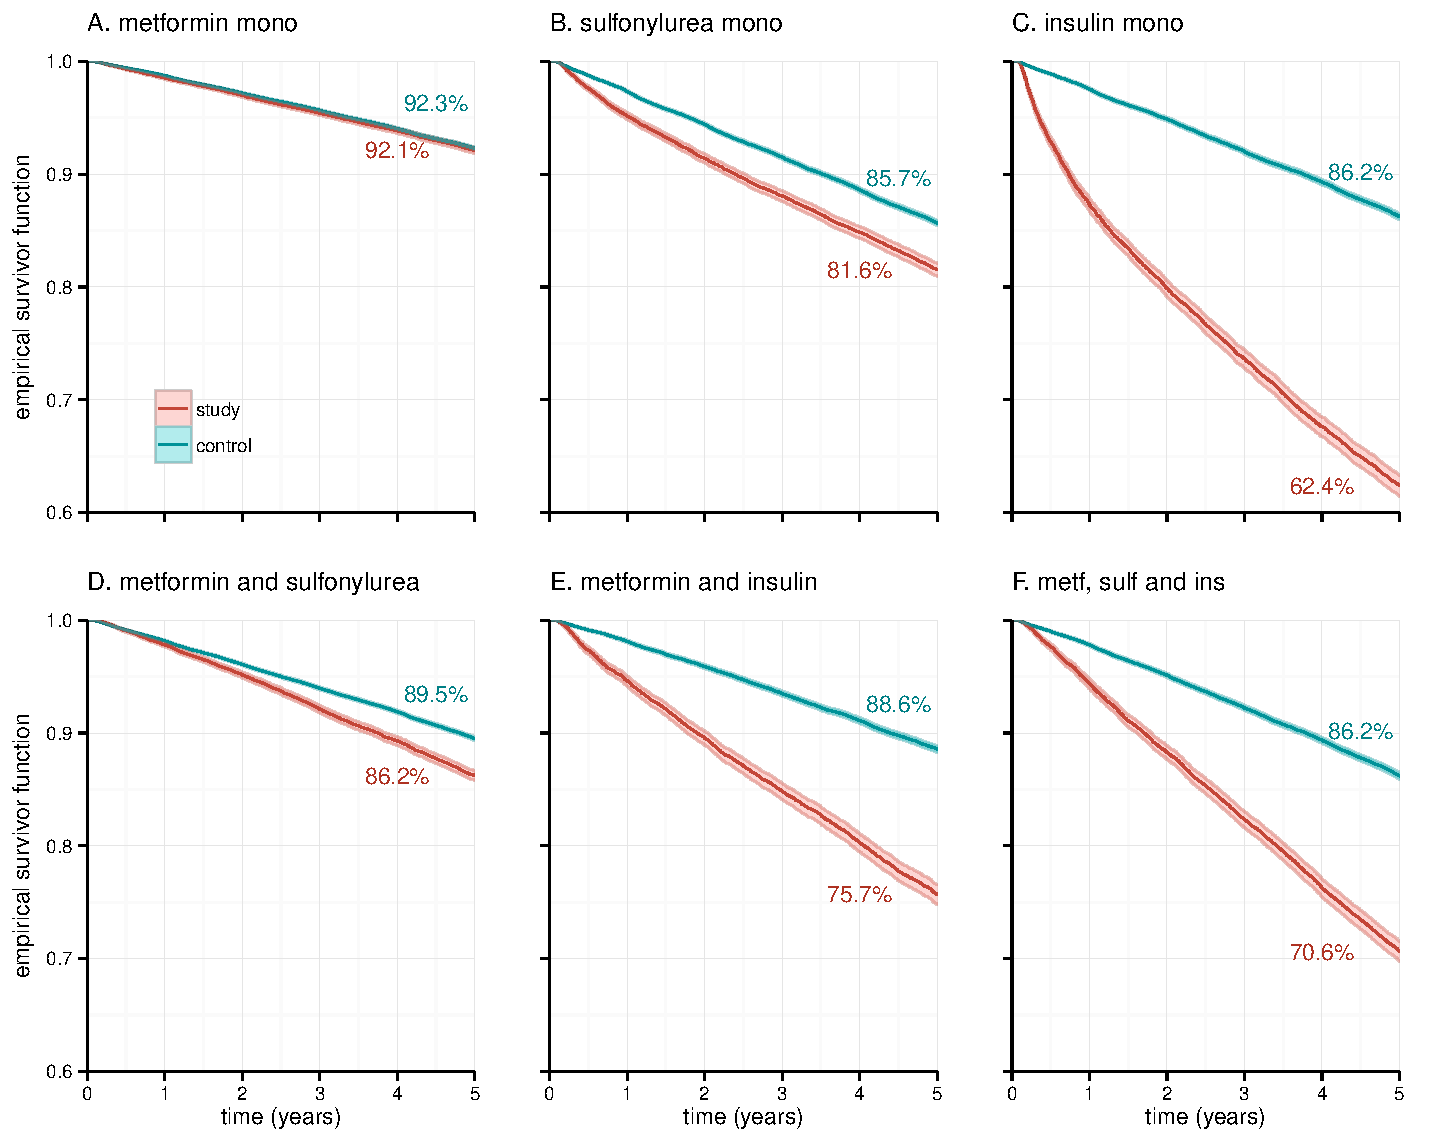
\includegraphics[width=\textwidth]{survival_curves.pdf}
  \caption{5-year survival for increasing age per cohort.} \label{fig:survival-curves}
\end{figure}

Comparable differences were seen in survival of patients without a history of cardiovascular (CV) events, with the lowest survival rates in therapies involving both insulin and SU (up to 29\% difference after 5 years) (Table~\ref{table:survival-results}). Patients with a history of CV events consistently exhibited lower survival than patients without a CV history, but excess mortality compared to matched controls was comparable for both subgroups. Of note, the survival of patients with a CV history on metformin monotherapy was not significantly different from the survival of the associated controls.  The observed survival benefit of metformin monotherapy disappeared in combination therapy cohorts (Table~\ref{table:survival-results}).

\begin{table}[!h]
\begin{tabular}{lcccl}
\toprule
			 & \multicolumn{4}{c}{no history of cardiovasular disease}		 \\\cline{2-5} 
			 & \multicolumn{2}{c}{5-year survival ($\%$)} 		& & \multicolumn{1}{c}{hazard ratio} \\\cline{2-3} \cline{5-5}
study cohort	& study cohort 				& control 	&	& \multicolumn{1}{c}{$\frac{study}{control}$} \\
\midrule
%\multicolumn{5}{l}{\textbf{overview categories}}	\\
%any OAD	or insulin 		& $85.9\ [85.6$--$86.1]$ & $90.9\ [90.8$--$91.0]$ & $p<0.001$ &  & $73.2\ [72.2$--$74.2]$ & $80.7\ [80.3$--$81.1]$ & $p<0.001$ \\
%any OAD					& $89.6\ [89.3$--$89.8]$ & $91.5\ [91.4$--$91.6]$ & $p<0.001$ &  & $80.8\ [79.7$--$81.8]$ & $81.9\ [81.5$--$82.4]$ & $p=0.024$ \\

%\multicolumn{5}{l}{\textbf{mono therapy}}	\\
metformin 				 & $92.6\ [92.3$--$92.9]$ & $92.9\ [92.8$--$93.0]$ & & $1.07$ $[1.02$--$1.11]$ \\
sulfonylurea 			& $82.5\ [81.9$--$83.1]$ & $86.5\ [86.3$--$86.8]$ & & $1.45$ $[1.40$--$1.52]$ $\bullet$ \\
insulin					& $63.9\ [62.9$--$64.9]$ & $88.1\ [87.8$--$88.3]$ & & $4.32$ $[4.14$--$4.51]$ $\bullet$ \\

%\multicolumn{5}{l}{\textbf{combination therapy}}	\\
metf+sulf				& $87.0\ [86.5$--$87.4]$ & $90.3\ [90.1$--$90.5]$ & & $1.40$ $[1.35$--$1.46]$ \\
metf+insulin			& $77.1\ [76.1$--$78.0]$ & $89.8\ [89.5$--$90.1]$ & & $2.71$ $[2.56$--$2.87]$ $\bullet$ \\
sulf+insulin			& $50.3\ [48.8$--$51.7]$ & $78.4\ [77.8$--$78.9]$ & & $3.07$ $[2.92$--$3.23]$ $\bullet$ \\
metf+sulf+insulin		& $71.5\ [70.5$--$72.5]$ & $87.5\ [87.2$--$87.8]$ & & $2.71$ $[2.58$--$2.85]$ \\
& \\
			 & \multicolumn{4}{c}{history of cardiovasular disease}		 \\\cline{2-5} 
			 & \multicolumn{2}{c}{5-year survival ($\%$)} 		& & \multicolumn{1}{c}{hazard ratio} \\\cline{2-3} \cline{5-5}
study cohort	& study cohort 				& control 	&	& \multicolumn{1}{c}{$\frac{study}{control}$} \\
\midrule
metformin 				 & $86.7\ [85.4$--$87.8]$ & $85.2\ [84.6$--$85.7]$ & & $0.92$ $[0.83$--$1.02]$ \\ % 0.0134941156118035 0.914200065217855
sulfonylurea 			        & $72.5\ [70.2$--$74.6]$ & $77.2\ [76.4$--$78.1]$ & & $1.35$ $[1.22$--$1.50]$ \\ % 2.36504826833794e-08 0.0480318297463539
insulin					& $56.1\ [53.9$--$58.3]$ & $78.6\ [77.9$--$79.3]$ & & $2.69$ $[2.49$--$2.90]$ \\ % 0 0.01384985104263

%\multicolumn{5}{l}{\textbf{combination therapy}}	\\
metf+sulf				& $79.1\ [77.4$--$80.7]$ & $81.8\ [81.1$--$82.5]$ & & $1.18$ $[1.07$--$1.30]$ $\bullet$ \\ % 0.1447394553308 0.00538876797400345
metf+insulin			& $69.2\ [66.9$--$71.4]$ & $82.7\ [81.8$--$83.5]$ & & $2.07$ $[1.87$--$2.30]$ \\ % 0.000117768936021667 0.938594402031259
sulf+insulin			& $48.8\ [46.2$--$51.3]$ & $74.3\ [73.3$--$75.2]$ & & $2.66$ $[2.44$--$2.89]$ \\ % 3.54578223642488e-05 0.0215754942151928
metf+sulf+insulin		& $67.4\ [65.5$--$69.3]$ & $81.5\ [80.8$--$82.2]$ & & $2.05$ $[1.89$--$2.23]$ \\ % 0.123550131268869 0.491309681508373
\bottomrule
\end{tabular}
\caption{Overview of survival for the study cohorts compared to a fully matched control cohort, stratified by cv history. The control group is sampled from the general population and matched for age, gender and use of statins, antihypertensives and antiplatelet drugs. For every patient in the study cohorts, 5 patients with completely matching profiles were used in control. $\bullet$ indicates that the proportional hazards assumption was rejected for the associated hazards ratio ($p<0.01$).} \label{table:survival-results}
\end{table}


\subsection{Age-dependent 5-year survival of individuals on different glucose lowering agents}
Figure~\ref{fig:survival-by-age} illustrates the 5-year survival of patients as a function of age at the start of follow-up. Compared to the general population, 5-year survival was lower at any age in all cohorts on glucose lowering monotherapy except the metformin monotherapy cohort, which exhibits comparable survival to the general population. At any certain age, survival was highest in patients on metformin, worse in patients on sulfonylurea, and worst in patients on insulin. In patients starting on combination therapy, survival was also lower at any age than associated controls. Again, if the regimen contains insulin, survival is worse at any age category, with or without sulfonylurea on board. 


\afterpage{%
    \clearpage% Flush earlier floats (otherwise order might not be correct)
    \thispagestyle{empty}% empty page style (?)
    \begin{landscape}% Landscape page
        \centering % Center table
\hspace{-0.2\textheight}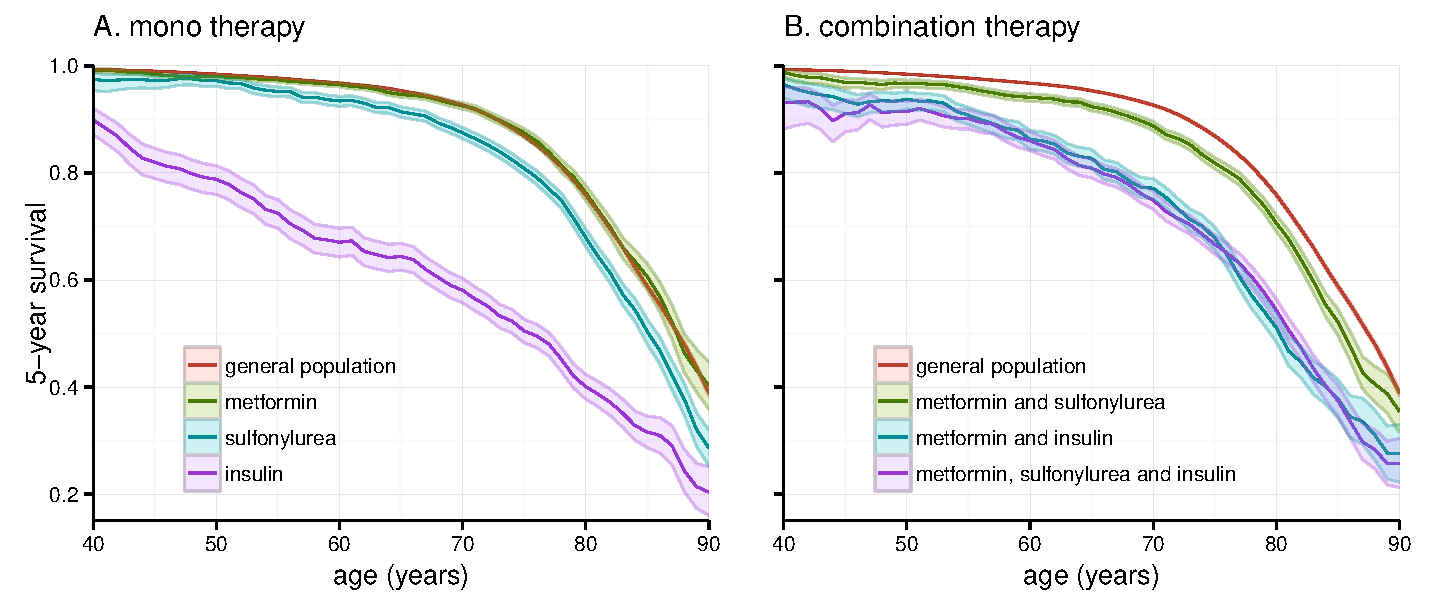
\includegraphics[width=1.7\textheight]{survival_by_age.pdf} \label{fig:survival-by-age}
\captionof{figure}{5-year survival for increasing age per cohort.}
\end{landscape}
\clearpage%
}

\afterpage{%
    \clearpage% Flush earlier floats (otherwise order might not be correct)
    \thispagestyle{empty}% empty page style (?)
    \begin{landscape}% Landscape page
        \centering % Center table
\hspace{-0.2\textheight}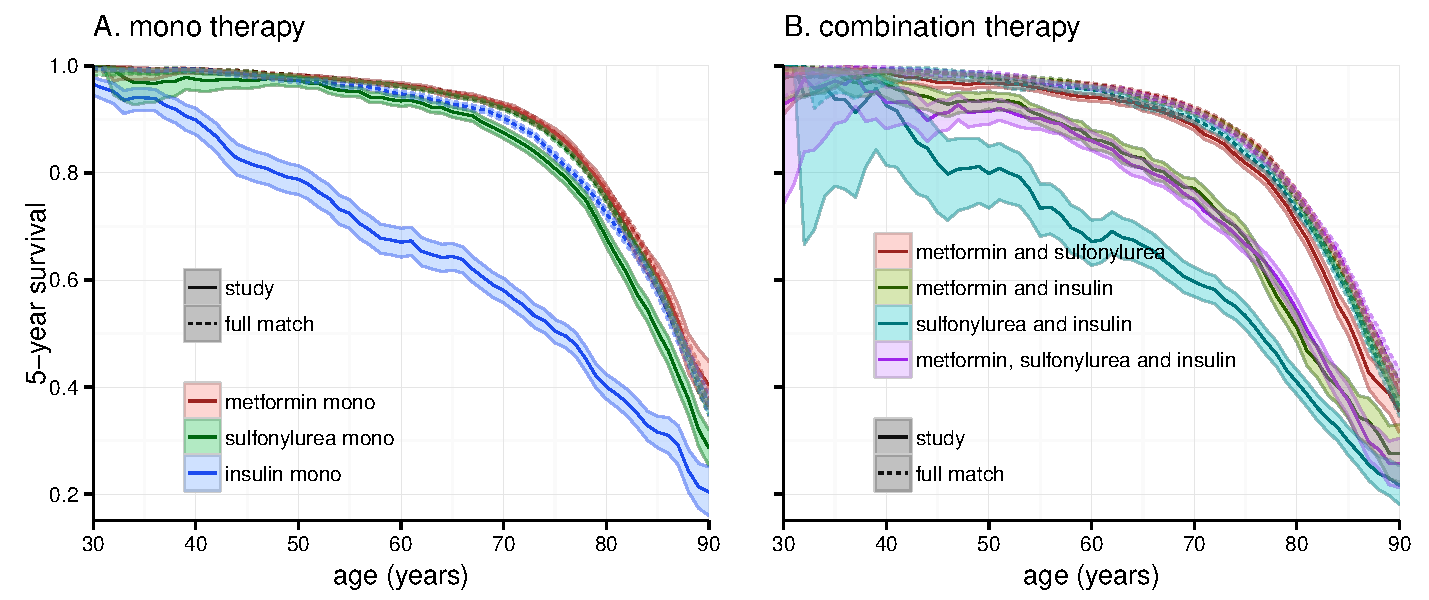
\includegraphics[width=1.7\textheight]{survival_by_age_matched.pdf} \label{fig:survival-by-age-matched}
\captionof{figure}{5-year survival for increasing age per cohort with matched controls.}
\end{landscape}
\clearpage%
}

The differences in survival at any age were slightly reduced when comparing to fully matched controls, though they remain large and statistically significant (illustrations are given in Figure~\ref{fig:survival-by-age-matched}). This reduction in excess mortality appears to be mainly attributable to the fact that the fully matched control groups have a higher frequency of prior cardiovascular events than the unmatched general population. 

Patients starting metformin monotherapy at a very young age (between 18 and 40 years; n=1,446; 83.3\% male) had a 5-year survival rate of 99.2\% $[98.4\%$--$99.6\%]$ compared to 99.3\% $[99.1\%$--$99.5\%]$ for fully matched controls (p=0.644). Of note, all females in this study group (n = 242) survived the entire follow-up. In the age category 18 to 40 years, the 5-year survival rate of patients on insulin monotherapy (n = 1,873) was reduced compared to fully matched controls (p < 0.001), with survival rates of 94.7\% $[93.4\%$--$95.6\%]$ and 99.5\% $[99.3\%$--$99.6\%]$ respectively. 

\subsection{Statins and survival in individuals on different glucose lowering therapy}
Survival was compared between patients with and without statins. Survival was consistently higher for patients that used statins in conjunction with GLA therapy (Table~\ref{table:survival-statins}), irrespective of CV history. The observed mortality rate when using statins along with GLAs was 57 to 64\% lower in patients without a history of CV disease and by 50 to 68\% in patients with a CV history, compared to patients using only GLAs.

\begin{table}[!h]	% hazard_ratio_2.R
\centering
\begin{tabular}{llcll}
\toprule
			 & \multicolumn{4}{c}{no history of cardiovasular disease}\\\cline{2-5}
			 & \multicolumn{2}{c}{5-year survival ($\%$)} 		& & \multicolumn{1}{c}{hazard ratio} \\\cline{2-3} \cline{5-5}
study cohort	& without statins 	& with statins 	&	& \multicolumn{1}{c}{$\frac{statins}{no\ statins}$} \\
\midrule

metformin               & $90.2\ [89.8$--$90.6]$ & $95.5\ [95.2$--$95.9]$ & & $0.43\ [0.39$--$0.47]$ $\bullet$ \\
sulfonylurea            & $76.9\ [76.1$--$77.8]$ & $91.7\ [91.0$--$92.4]$ & & $0.36\ [0.32$--$0.40]$ $\bullet$ \\
insulin                 & $59.6\ [58.4$--$60.8]$ & $77.3\ [75.4$--$79.0]$ & & $0.37\ [0.33$--$0.41]$ $\bullet$ \\

metf+sulf               & $82.5\ [81.8$--$83.2]$ & $92.6\ [92.0$--$93.1]$ & & $0.42\ [0.38$--$0.46]$ $\bullet$ \\
metf+insulin            & $68.2\ [66.7$--$69.6]$ & $86.8\ [85.7$--$87.9]$ & & $0.39\ [0.35$--$0.44]$ \\
sulf+insulin            & $41.3\ [39.6$--$43.1]$ & $69.9\ [67.4$--$72.3]$ & & $0.43\ [0.38$--$0.48]$ \\
metf+sulf+insulin       & $61.5\ [60.0$--$62.9]$ & $83.4\ [82.1$--$84.5]$ & & $0.43\ [0.39$--$0.48]$ $\bullet$ \\
& \\
			 & \multicolumn{4}{c}{history of cardiovasular disease}\\\cline{2-5}
			 & \multicolumn{2}{c}{5-year survival ($\%$)} 		& & \multicolumn{1}{c}{hazard ratio} \\\cline{2-3} \cline{5-5}
study cohort	& without statins 	& with statins 	&	& \multicolumn{1}{c}{$\frac{statins}{no\ statins}$} \\
\midrule
metformin               & $71.3\ [67.5$--$74.6]$ & $90.6\ [89.4$--$91.7]$ & & $0.36\ [0.29$--$0.45]$ \\ % 0.58 0.898
sulfonylurea            & $53.1\ [48.8$--$57.2]$ & $82.5\ [80.1$--$84.6]$ & & $0.32\ [0.26$--$0.40]$ \\ % 0.06 0.239
insulin                 & $40.5\ [37.0$--$43.9]$ & $66.5\ [63.7$--$69.1]$ & & $0.45\ [0.39$--$0.53]$ \\ % 0.001 0.606

metf+sulf               & $62.8\ [58.8$--$66.5]$ & $85.0\ [83.2$--$86.6]$ & & $0.42\ [0.34$--$0.51]$ $\bullet$ \\ % 0.03 0.262
metf+insulin            & $46.7\ [42.0$--$51.2]$ & $77.9\ [75.4$--$80.2]$ & & $0.40\ [0.33$--$0.49]$ \\ % 0.025 0.023
sulf+insulin            & $32.3\ [28.6$--$36.0]$ & $60.8\ [57.4$--$63.9]$ & & $0.50\ [0.42$--$0.59]$ \\ % 0.124 0.317
metf+sulf+insulin       & $46.6\ [42.8$--$50.3]$ & $76.6\ [74.4$--$78.6]$ & & $0.42\ [0.35$--$0.49]$ \\ % 0.004 0.197
\bottomrule
\end{tabular}
\caption{Analysis of the effect of statins within each study cohort. Presented hazard ratios are associated to the fraction of follow-up on statins. Patients are classified as statin users if they were on statins for at least half the follow-up. The proportional hazards models used here control for age, gender, use of antihypertensive and antiplatelet drugs and an age-gender interaction. $\bullet$ indicates that the proportional hazards assumption was rejected for the associated hazards ratio ($p<0.01$).} \label{table:survival-statins} % http://en.wikipedia.org/wiki/Controlling_for_a_variable
\end{table}

In a second analysis, cohorts in which all patients on glucose lowering therapy were taking statins were compared to the general age and gender matched population. Patients on metformin monotherapy (with and without a CV history) and sulfonylurea mono (without CV history) that were also taking statins exhibited higher survival rates than age and gender matched control groups without glucose lowering therapy  (of which resp. only 32,4\%, 24.7\%, and 29.9\% were taking statins during the majority of the follow-up). Patients on the combination of MET and SU and statins had the same survival rate than their controls, irrespective of CV history (Table~\ref{table:survival-statins-hrs}).
 
\begin{table}[!h]	% hazard_ratios_1.R
\centering
\begin{tabular}{lll}
\toprule
study cohort	& no history of CVD		& history of CVD \\%\cline{2-3} \cline{5-6}
%study cohort	& \multicolumn{1}{c}{study} & \multicolumn{1}{c}{study + statins}  & & \multicolumn{1}{c}{study} & \multicolumn{1}{c}{study + statins} \\
\midrule

%\multicolumn{5}{l}{\textbf{mono therapy}}	\\
metformin 				& $0.66\ [0.61$--$0.71]$ $\bullet$ & $0.67\ [0.58$--$0.78]$ \\ % 0.003 0.001 0.554 0.566
sulfonylurea 			& $0.88\ [0.80$--$0.97]$ & $0.95\ [0.81$--$1.12]$ \\ % 0 0.143 0 0.933
insulin					& $2.84\ [2.53$--$3.19]$ $\bullet$ & $2.12\ [1.83$--$2.47]$ \\ % 0 0.003 0.036 0.654

%\multicolumn{5}{l}{\textbf{combination therapy}}	\\
metf+sulf				& $0.91\ [0.84$--$0.99]$ $\bullet$ &  $0.96\ [0.84$--$1.11]$ $\bullet$ \\ % 0.319 0 0.001 0
metf+insulin			& $1.91\ [1.71$--$2.14]$ & $1.67\ [1.37$--$2.03]$ \\ % 0 0.259 0.543 0.486
sulf+insulin			& $2.40\ [2.13$--$2.71]$ & $2.43\ [2.07$--$2.87]$ \\ % 0 0.142 0.472 0.792
metf+sulf+insulin		& $1.83\ [1.66$--$2.01]$ & $1.44\ [1.23$--$1.69]$ \\ % 0.216 0.051 0.618 0.472
\bottomrule
\end{tabular}
\caption{Hazard ratios between statin users in the study group a control group matched for age and gender. 
The remaining characteristics of the control groups used here follow the distribution of the total NACM member population (after matching for age and gender).
The proportional hazard models used to compute these hazard ratios control for age, gender, the use of antihypertensive and antiplatelet drugs and an age-gender interaction. $\bullet$ indicates that the proportional hazards assumption was rejected for the associated hazards ratio ($p<0.01$).} \label{table:survival-statins-hrs}
\end{table}

\section{Conclusions}
The main objective of this large controlled cohort study was to investigate the survival of patients on various glucose lowering therapies in comparison to a reference population with similar observable characteristics. It was found that 5-year survival rates vary between glucose lowering therapies, at least partly driven by the risk profile of the individuals themselves, and substantially influenced by the intake of statins and the age at the start of GLA therapy.

Increased 5-year mortality rates were observed in patients on GLAs compared to matched references not on GLAs. This confirms the study of Bannister et al. \citep{s9} showing an increased mortality in patients on SU monotherapy and extends the evidence to other groups on insulin monotherapy and different combination therapies. Although we did not see a better survival rate in patients on metformin monotherapy, our data show that these patients have similar survival rates compared to matched controls, especially if a positive history of CV disease is present. 

Our study confirms data from many other observational studies that patients on metformin monotherapy have a lower mortality risk than patients on other glucose lowering therapy \citep{s3,s4,s5,s6,s7,s8}, characterized by reduced excess mortality compared to matched controls. This study does determine whether this excess mortality of patients on SU and insulin is mainly caused by the vulnerability of the background population or by negative properties of the therapies themselves. The extra mortality risk can, at least partially, be explained by the risk profile of the individuals themselves and not by using SU or insulin per se. First of all, this might reflect the progressive nature of type 2 diabetes such that patients with less pronounced hyperglycemia are started on metformin monotherapy whereas uncontrolled patients are started on insulin or combination therapies including SU. Age is another important independent predictor of mortality and can explain why younger patient groups (i.e. metformin mono) have better survival rates than older patient groups (i.e. SU mono). Age however does not explain the lower survival rates in younger patients on insulin monotherapy and survival differences throughout all age categories. A positive history of cardiovascular events also increases the background risk of our populations and explains the lower survival rates in any study cohort with a positive CV history.  As in Morgan et al. \citep{s7}, a combination of several other elements will probably play a role such as hypertension and factors that were not available in our study such as presence of chronic kidney disease and albuminuria, the level of glycemic control, smoking and heart failure.

Data from literature are conflicting concerning differences between agents. On the one hand several studies report no difference in survival when comparing metformin with SU \citep{s18,s19,s20} or SU with insulin \citep{s19}. Also in the ORIGIN trial, insulin glargine was not associated with higher mortality rates than controls \citep{s21} despite the lower use of metformin in the insulin glargine group. On the other hand, many clinical and observational studies have indicated an increased mortality risk associated with the use of SU and insulin compared to metformin \citep{s3,s4,s5,s6,s7,s8}, although differences were shown to depend on the type of SU \citep{s22,s23}, and the dose of insulin \citep{s24} used. In fact only a well-controlled RCT with sufficient power comparing different treatment strategies might answer this question, but it is very unlikely that these RCT's will ever be undertaken. Observational studies are in that view considered complementary as they do not omit patients on the basis of strict criteria and will usually have enough follow-up time to evaluate hard endpoints such as mortality risk. 

This study is the first to show a beneficial impact of intake of statins on real-life survival data in a large population study of patients on glucose lowering therapy. This is not unexpected, since available evidence from RCT's convincingly showed beneficial effect of statins on survival and prevention of cardiovascular events in secondary prevention (reviewed in \citep{s25}). Data in primary prevention are scarce with the only RCT in diabetic patients lacking power to show an overall mortality benefit \citep{s26}. Our trial shows a beneficial effect of statins in patients with diabetes, both in primary and secondary prevention, with mortality risks being 60 to 80\% lower independent of the type of glucose lowering therapy or presence of a CV disease history. Of note, patients taking statins in combination with metformin or SU monotherapy even showed better survival than the general population. 

An asset of this study was the use of health expenditure records to assess the survival of patients on various glucose lowering therapies in comparison with a similar reference cohort from the general population. Claims records constitute a valuable source of information for observational epidemiological studies by embedding long-term longitudinal medical information of a large number of patients. Additionally, claims records aggregate proxies of medical information from various caregivers into a complete patient-wide overview which is often unavailable to individual caregivers and other medical stakeholders. 

Through exact pair-wise matching of the reference cohort and regression adjustment in the proportional hazards models we were able to exclude important observable confounders in comparisons of the study cohorts with their respective references \citep{s27}. Having access to a large population from which to sample control subjects allowed us to find references with exact matches on key confounding variables. Matching on these observable factors excludes the confounding effect and yields an efficiency gain \citep{s28}. Some residual confounding resulting from uncontrolled and unobservable factors may remain.
Our study also has limitations. While there are considerable benefits in using claims data for epidemiological research, the absence of detailed clinical parameters prohibits causal inference because we could not control for level of glycemic control (e.g., fasting blood glucose or HbA1c), BMI, or other modifiable cardiovascular risk factors (e.g., smoking). However, we controlled for age, sex, concomitant medication, and presence of history of CV disease. Due to its observational nature our study remains susceptible to confounding by indication \citep{s29,s30,s31}. Therefore our study is not suitable to compare GLA therapies directly as the patients' underlying conditions yield indications for their treatment, preventing comparisons \citep{s29,s32}. 

We conclude that 5-year survival in patients on glucose lowering therapy is lower than in matched controls except for metformin monotherapy. Intake of metformin is associated with lowest 5-year mortality. In all groups, the intake of statins was associated with a reduced mortality rate.


% vim: tw=70 nocindent expandtab foldmethod=marker foldmarker={{{}{,}{}}}
